\documentclass[t]{beamer}
\usetheme{Copenhagen}
\setbeamertemplate{headline}{} % remove toc from headers
\beamertemplatenavigationsymbolsempty

\usepackage{amsmath, array, tikz, bm, pgfplots, tcolorbox, graphicx, venndiagram, color, colortbl}
\pgfplotsset{compat = 1.16}
\usepgfplotslibrary{statistics}
\usetikzlibrary{trees}

\title{Speed Counting}
\author{}
\date{}

\AtBeginSection[]
{
  \begin{frame}
    \frametitle{Objectives}
    \tableofcontents[currentsection]
  \end{frame}
}

\begin{document}

\begin{frame} 
\maketitle
\end{frame}

\section{Use the Fundamental Counting Rule}

\begin{frame}{Example 1}
For a special at a restaurant, you can choose between 3 appetizers, 4 entrees, and 2 desserts. If you select one item from each category (appetizer, entree, and dessert), how many different meals can you create?	\newline\\	\pause

Let's call the appetizers A, B, and C. \newline \pause
Let's call the entrees D, E, F, and G. \newline \pause
Let's call the desserts H and I.	\newline\\	\pause

With appetizer A: ADH, ADI, AEH, AEI, AFH, AFI, AGH, AGI \newline \pause
With appetizer B: BDH, BDI, BEH, BEI, BFH, BFI, BGH, BGI \newline \pause
With appetizer C: CDH, CDI, CEH, CEI, CFH, CFI, CGH, CGI \newline\\ \pause

For a total of 24 possible different meals.
\end{frame}

\begin{frame}{Fundamental Counting Rule}
If event $A$ can occur in $a$ different ways and event $B$ can occur in $b$ different ways, then the total number of ways both events can occur is $ab$ ways.	\newline\\	\pause

This can be generalized to multiple events, such as those in example 1: $3 \times 4 \times 2 = 24$
\end{frame}


\section{Understand factorial notation}

\begin{frame}{Example 2}
A baseball lineup consists of 9 players. How many different lineups using all 9 players on a team exist?	\newline\\	\pause

Using the Fundamental Counting Rule with 9 positions:	\newline\\	\pause


\begin{tabular}{|c|c|c|c|c|c|c|}
1st pos. &	2nd pos. &	3rd pos. &	$\dots$ & 7th pos.	&	8th pos. &	9th pos.  \\ \hline
\onslide<4->{9} & \onslide<5->{8} & \onslide<6->{7} & \onslide<7->{$\dots$} & \onslide<8->{3} &\onslide<9->{2} & \onslide<10->{1} \\
\end{tabular}
\vspace{10pt}
\onslide<11->{\[9 \times 8 \times 7 \times \cdots \times 2 \times 1 \onslide<12->{= 362,880 \text{ unique lineups}}\]}

\end{frame}

\begin{frame}{Factorial Notation}
Rather than write out all the numbers from 9 to 1 and then multiplying them, mathematicians created {\color{blue}\textbf{factorial notation}} to expedite the process.	

\onslide<2->{\[9! = 9 \times 8 \times 7 \times \cdots \times 3 \times 2 \times 1 = 362,880\]}

\onslide<3->{In general, for a positive integer $n$, \[n! = n(n-1)(n-2) \cdot \cdots \cdot 3(2)(1)\]}
\onslide<4->{with $0! = 1$}
\end{frame}

\begin{frame}{Factorial Growth}
Factorial values grow very quickly:
\begin{align*}
2! &= 2(1) &= 2 \\
3! &= 3(2)(1) &=6 \\
4! &= 4(3)(2)(1) &= 24 \\
5! &= 5(4)(3)(2)(1) &= 120 \\
6! &= 6(5)(4)(3)(2)(1) &= 720	\\
7! &= 7(6)(5)(4)(3)(2)(1) &= 5,040
\end{align*}
\end{frame}

\begin{frame}{Example 3}
How many ways are there to arrange 5 books on a shelf?
\onslide<2->{\[5! = 120 \text{ different arrangements}\]}
\end{frame}

\section{Find permutations of objects}

\begin{frame}{Example 4}
Five people are competing for three prizes: \$1,000, \$500, and \$100. How many different ways can the prizes be awarded?	\newline\\
\begin{center}
\onslide<2->{
	\begin{tabular}{|c|c|c|}
	\$1,000 		&		\$500			&	\$100			\\	\hline
	\onslide<3->{5}	&	\onslide<4->{4}		&	\onslide<5->{3}	\\
	\end{tabular}
}
\end{center}
\onslide<6->{Using the Fundamental Counting Rule:
			\[ 5 \times 4 \times 3 = 60\text{ different ways}\]}
\end{frame}

\begin{frame}{Takeaways from Example 4}
We had more contestants available to win prizes than we had prizes available. We could have had an equal number of contestants and prizes, but we can't have more prizes available than contestants. \newline\\	\pause

If we had 10,000 contestants and 75 prizes, we would have a lot of multiplying to do.	\newline\\	\pause

So is there an easy way to do this if that's the case?	\newline\\	\pause

Yes, and that is where {\color{blue}\textbf{permutations}} come into play.
\end{frame}

\begin{frame}{Example 5}
How many ways are there to award gold, silver, and bronze medals to 8 contestants?	\newline\\
\begin{center}
\onslide<2->{
	\begin{tabular}{|c|c|c|}
	Gold 		&		Silver			&	Bronze			\\	\hline
	\onslide<3->{8}	&	\onslide<4->{7}		&	\onslide<5->{6}	\\
	\end{tabular}
}
\end{center}
\onslide<6->{Using the Fundamental Counting Rule:
			\[ 8 \times 7 \times 6 = 336\text{ different ways}\]}
\end{frame}

\begin{frame}{Example 5}
\[\alert{8} \times \alert{7} \times \alert{6} \times \dots \times 2 \times 1\]
\end{frame}

\begin{frame}{Example 5}
\[\frac{\alert{8} \times \alert{7} \times \alert{6} \times 5 \times 4 \times 3 \times 2 \times 1}{5 \times 4 \times 3 \times 2 \times 1}\]
\end{frame}

\begin{frame}{Example 5}
\[\alert{8} \times \alert{7} \times \alert{6} = 336\]
\end{frame}

\begin{frame}{Permutations}
If there are $n$ items available and we take $r$ at a time, then the total number of permutations is given by 
\[_nP_r = \frac{n!}{(n-r)!}\]

with $n \geq r$	\newline\\

\pause With permutations, the order in which an item is selected matters.
\end{frame}

\begin{frame}{Knowing to Use Permutations}
Permutations
\begin{itemize}
	\item<+-> Offering various prizes
	\item<+-> Running a race
	\item<+-> Assigning officer positions
	\item<+-> Combination locks and passwords
\end{itemize}
\end{frame}

\begin{frame}{Example 6}
How many ways are there of selecting a president, vice president, secretary, and treasurer out of a pool of 10 candidates?	\newline\\	\pause
Order matters.	\newline	\pause
We have $n = 10$ items to choose from.	\newline	\pause
We are filling $r = 4$ positions at a time.	\newline	
\begin{align*}
\onslide<5->{_{10}P_4 &= \frac{10!}{(10-4)!}} \\[8pt]
\onslide<6->{&= \frac{10!}{6!}} \\[8pt]
\onslide<7->{&= 5,040}
\end{align*}
\end{frame}

\section{Find combinations of objects}

\begin{frame}{Combinations}
With permutations, order selection mattered, so 
\begin{center}
ABC, ACB, BAC, BCA, CAB, and CBA
\end{center}
were all different.	\newline\\	\pause

With combinations, selection order does not matter, so there is no distinction among the orderings above. So,
\begin{center}
ABC, ACB, BAC, BCA, CAB, and CBA
\end{center}
are all the same.
\end{frame}

\begin{frame}{Combinations}
Notice that there are 6, or $3!$, arrangements of the letters A, B, and C. \newline\\	\pause

This can help us develop the formula for finding the number of combinations of $n$ items taken $r$ at a time.
\end{frame}

\begin{frame}{Example 7}
Five people are competing for three equal prizes. How many ways can the prizes be awarded?	\newline\\	\pause

If order mattered, there would be $_5P_3 = 60$ different possibilities:
\begin{center}
\begin{tabular}{ccccccc}
ABC & ABD & ABE & ACB & ACD & ACE & $\dots$ \\
BAC & BAD & BAE & BCA & BCD & BCE & $\dots$ \\
$\vdots$ & $\vdots$ & $\vdots$ & $\vdots$ & $\vdots$ & $\vdots$ & $\dots$ 
\end{tabular}
\end{center}
\end{frame}

\begin{frame}{Example 7}
Since ABC is the same as ACB, BAC, BCA, CAB, and CBA in the eyes of combinations, we can divide our permutation result of 60 by 3! to get \alert{10 combinations}:

\begin{center}
\begin{tabular}{ccccc}
ABC & ABD & ABE & ACD & ACE \\
ADE & BCD & BCE & BDE & CDE \\
\end{tabular}
\end{center}
\end{frame}

\begin{frame}{Combinations}
If we have $n$ items available and we take $r$ at a time {\color{blue}\textbf{without regard to order of selection}}, then the total number of possible combinations are

\onslide<2->{\[_nC_r = \frac{n!}{r!(n-r)!} \onslide<3->{= \binom{n}{r}}\]}

\onslide<4->{
	Combinations
	\begin{itemize}
		\item<5-> Awarding equal prizes
		\item<6-> Combinations (not the lock though)
		\item<7-> Committees
	\end{itemize}
}
\end{frame}

\begin{frame}{Example 8}
A committee of 5 is to be formed from a pool of 12 potential candidates. How many committees are possible?	\newline\\	
\onslide<2->{We have $n=12$ candidates to choose from} \newline
\onslide<3->{We are selecting $r=5$ at a time}
\begin{align*}
\onslide<4->{_{12}C_5 &= \frac{12!}{5!(12-5)!}}	\\[10pt]
\onslide<5->{&= 792}
\end{align*}
\end{frame}

\begin{frame}{Example 9}
A committee of 5 is to be formed from a pool of 12 potential candidates. The committee is to be made up of 3 managers and 2 accountants. If there are 8 managers and 4 accountants available, how many committees can be formed?	\newline\\
\onslide<2->{We need to make sure 3 of the positions are managers and 2 of the positions are accountants.} \newline\\
\onslide<3->{Thus, we must blend the Fundamental Counting Rule with combinations.}	
\end{frame}

\begin{frame}{Example 9}
\begin{center}
\setlength{\extrarowheight}{6pt}
\begin{tabular}{ccc}
Select 3 managers from 8 & $\times$ & Select 2 accountants from 4 \\ \hline
\onslide<2->{$_8C_3$} & $\times$ & \onslide<3->{$_4C_2$} \\
\onslide<4->{56} & $\times$ & \onslide<5->{6} \\
\end{tabular}
\end{center}
\onslide<6->{There are 336 ways to do this.}
\end{frame}

\begin{frame}{Example 10}
Starting at point $A$ and only moving right or up, how many paths are there to get to point $B$?	
\begin{center}
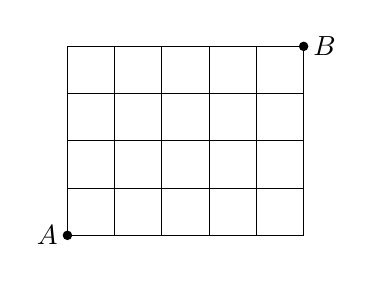
\begin{tikzpicture}[scale=0.6]
\draw (0,0) grid (5,4);
\draw [fill=black] (0,0) circle [radius=2.5pt] node [left] {$A$};
\draw [fill=black] (5,4) circle [radius=2.5pt] node [right] {$B$};
\end{tikzpicture}
\end{center}
\onslide<2->{You have to go right a total of 5 spaces and up a total of 4 spaces.} \newline\\
\onslide<3->{One example of such a path is UURURRRUR}
\end{frame}

\begin{frame}{Example 10}
Out of the 9 letters, we need 5 Rs and 4 Us. This can be solved using the Fundamental Counting Rule and combinations.	\pause
\begin{center}
\setlength{\extrarowheight}{6pt}
\begin{tabular}{ccc}
Pick 5 Rs from 9 letters & $\times$ & Pick 4 Us from \alert{the remaining} 4 letters	\\	\hline
\onslide<3->{$_9C_5$} & $\times$ & \onslide<4->{$_4C_4$} \\
\onslide<5->{126} & $\times$ & \onslide<6->{1} \\
\end{tabular}
\end{center}
\onslide<7->{There are 126 ways to do this.}
\end{frame}

\begin{frame}{Example 11}
How many ways can 20 people on a youth center basketball team be grouped into 6 centers, 4 shooting guards, 3 small forwards, 2 power forwards, and 5 point guards be assigned? \newline\\	\pause

\begin{center}
\begin{tabular}{cc}
For the centers, we have $n=20$ and $r=6$	&	$_{20}C_6$ 	\\ \pause
Shooting guards: $n=14$ and $r=4$:			&	$_{14}C_4$ 	\\ \pause
Small forwards: $n=10$ and $r=3$:			& 	$_{10}C_3$ 	\\ \pause
Power forwards: $n=7$ and $r = 2$: 			&	$_7C_2$    	\\ \pause
Point guards: $n=5$ and $r=5$: 				&	$_5C_5$		\\ \pause
\end{tabular}
\end{center}
\[_{20}C_6 \cdot _{14}C_4 \cdot _{10}C_3 \cdot _7C_2 \cdot _5C_5 = 97,772,875,200\]
\end{frame}

\begin{frame}{Example 11: Alternative Approach}
We can use the following formula to make quicker work of a problem like the previous example.	\newline\\	\pause

\[ \frac{n!}{r_1!r_2!r_3!\dots r_k!} \]	\bigskip

where $r_1 + r_2 + r_3 + \cdots + r_k = n$	\newline\\	\pause

\[\frac{20!}{6! \cdot 4! \cdot 3! \cdot 2! \cdot 5!} = 97,772,875,200\]
\end{frame}

\section{Find probabilities using counting techniques}

\begin{frame}{Counting and Probability}
We can use counting techniques to find the total number of outcomes we want to happen (numerator) and also to find the total number of possible outcomes (denominator)
\end{frame}

\begin{frame}{Example 12}
(a) \quad A combination lock has 3 dials with 10 digits each. What is the probability of guessing the combination on the first attempt?	\newline\\	\pause

Total number of possible outcomes (denominator): $10 \cdot 10 \cdot 10$	\newline\\	\pause
Total number of outcomes we want (numerator): 1	\newline\\	\pause

\[P(\text{guess correctly}) = \frac{1}{1,000}\]
\end{frame}

\begin{frame}{Example 12}
(b) \quad What is the probability of the previous example if each of the digits must be unique?	\newline\\	\pause

Total number of possible outcomes (denominator): $_{10}P_3$	\newline\\	\pause
Total number of outcomes we want (numerator): 1	\newline\\	\pause

\[P(\text{guess correctly}) = \frac{1}{720}\]
\end{frame}

\begin{frame}{Example 13}
In a state lottery, you pick 6 numbers from a possible 49 numbers and win a prize if you match at least 4 of the 6 numbers.	\newline\\

(a) \quad What is the probability of matching 4 out of the 6 numbers?	\newline\\ \pause
Total number of possible outcomes (denominator): $_{49}C_6$ \newline\\	\pause
Total number of outcomes we want (numerator): 
\begin{center}
\setlength{\extrarowheight}{6pt}
\begin{tabular}{ccc}
Select 4 winning nos. from 6 & $\times$ & Select 2 losing nos. from 43 \\ \hline
\onslide<4->{$_{6}C_4$} & $\times$ & \onslide<5->{$_{43}C_2$} \\
\end{tabular}
\end{center}
\end{frame}

\begin{frame}{Example 13a}

\[\frac{_{6}C_4 \times _{43}C_2}{_{49}C_6}\]	\pause
\[\approx 0.097\%\]


\end{frame}

\begin{frame}{Example 13}
(b) \quad What is the probability of getting a losing lottery ticket?	\newline\\	\pause
You have a losing ticket if you matched 3 numbers or less.	\newline\\	\pause
Since we already calculated the probability of getting 4 matches, we can continue up to 6 matches and then use the {\color{blue}\textbf{Complement Rule}}:	\newline\\	\pause

\begin{align*}
P(\text{losing ticket}) &= 1 - P(\text{winning ticket})	\\
\onslide<3->{&= 1 - P(\text{4 matches OR 5 matches OR 6 matches})} \\
\onslide<4->{&= 1 - \left(P(\text{4 matches})+ P(\text{5 matches}) + P(\text{6 matches})\right)}
\end{align*}
\end{frame}

\begin{frame}{Example 13b}
$P(4) = \dfrac{_{6}C_4 \times _{43}C_2}{_{49}C_6}$	\\[18pt]	\pause
$P(5) = \dfrac{_{6}C_5 \times _{43}C_1}{_{49}C_6}$	\\[18pt]	\pause
$P(6) = \dfrac{_{6}C_6 \times _{43}C_0}{_{49}C_6}$	\\[18pt]	\pause
$1-\left(P(4) + P(5) + P(6)\right)$					\\[18pt]	\pause
$99.90\%$ chance of purchasing a losing ticket.
\end{frame}

\end{document}